\documentclass[tikz, border=1pt]{standalone}
\pdfoutput=1 % if your are submitting a pdflatex (i.e. if you have
             % images in pdf, png or jpg format)

\usepackage{graphicx}

% Use the tikz package
\usepackage{tikz}
\usetikzlibrary{decorations}


\begin{document}

	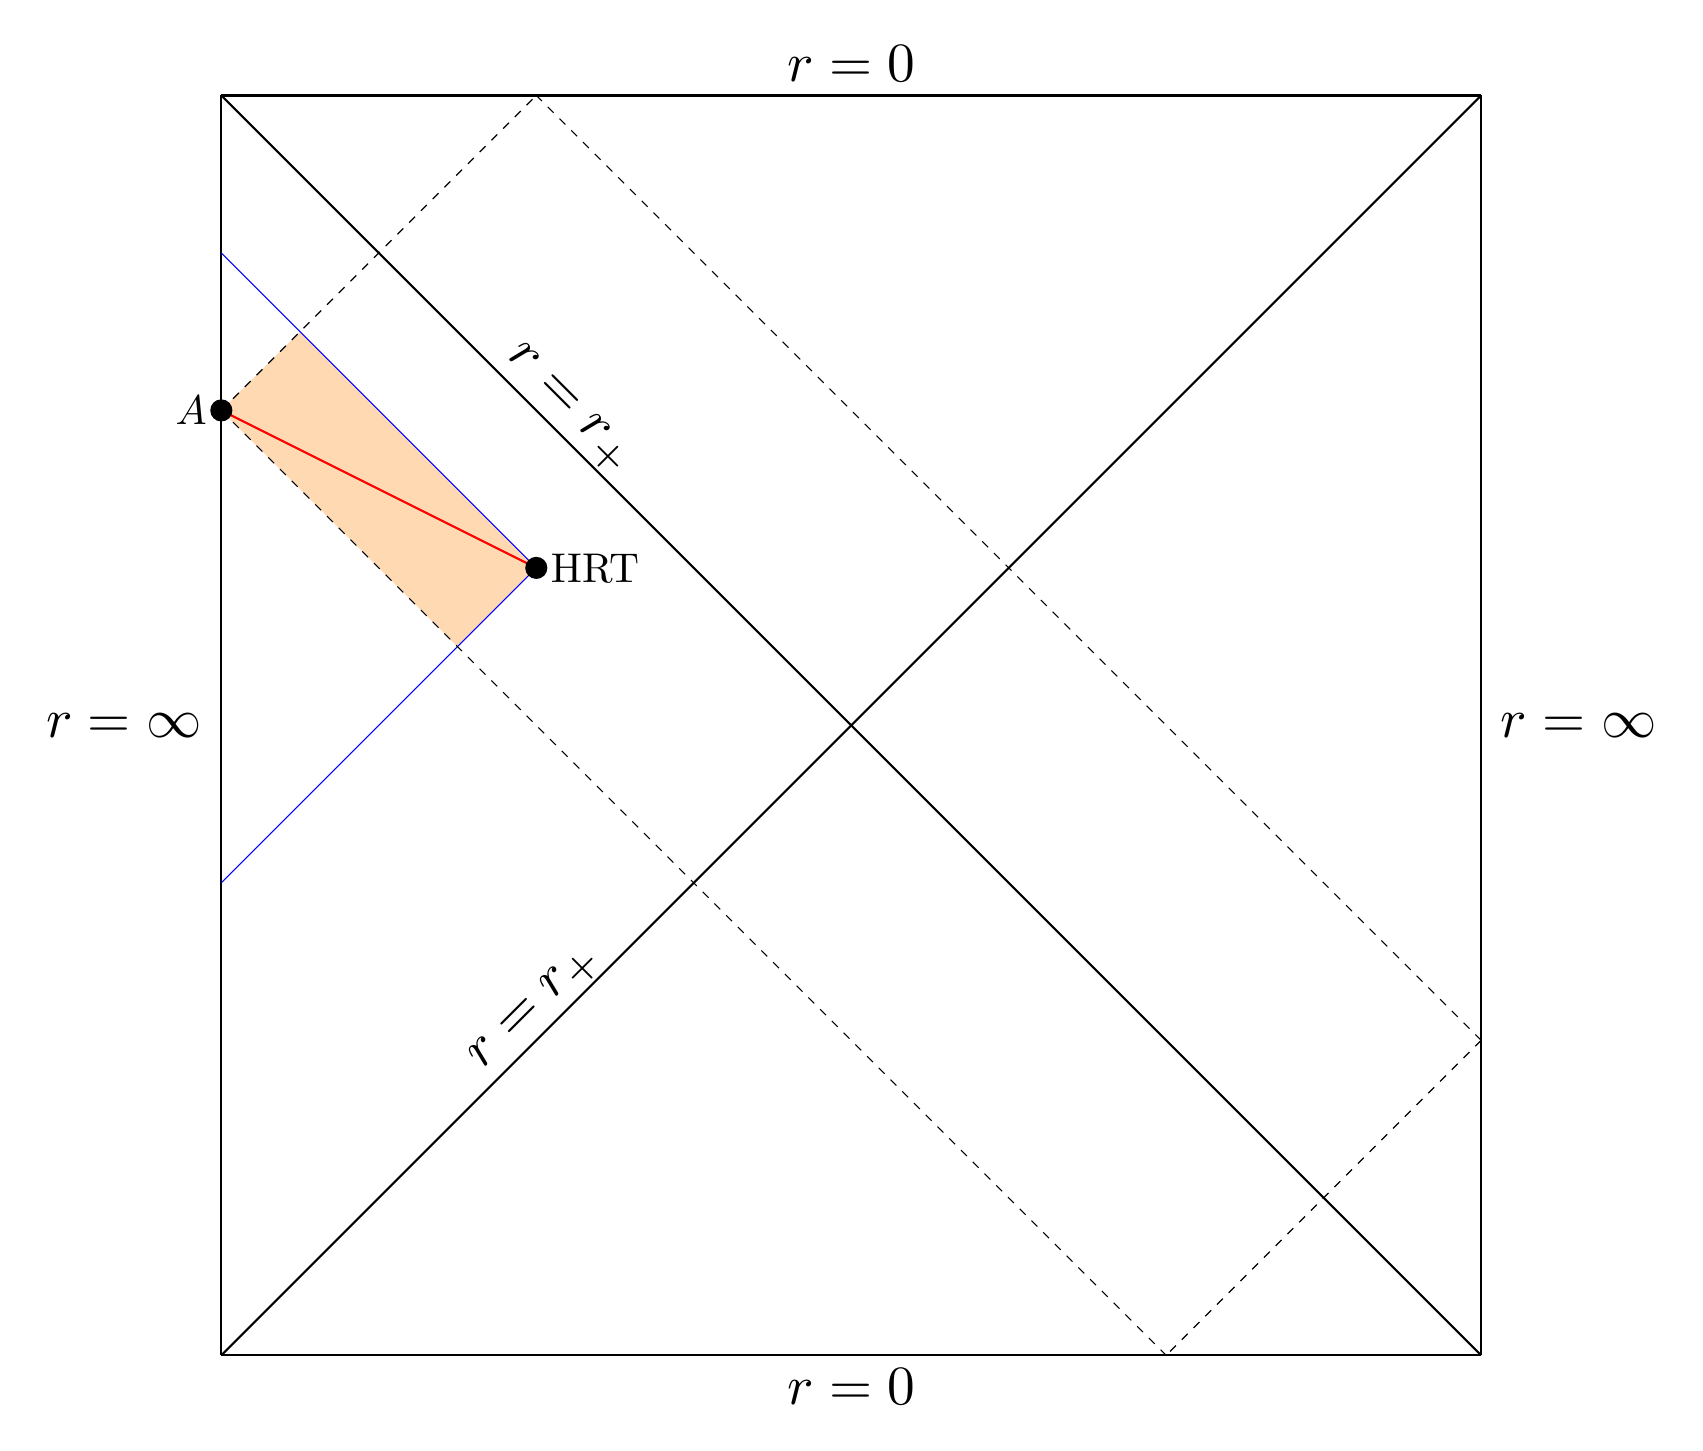
\begin{tikzpicture}[scale=4]
	
		% Fill in intersection
		\fill[orange!30!white] (0,3) -- (0.75,2.25) -- (1,2.5) -- (0.25, 3.25) -- (0,3) ;
        
        % Black hole axes
        \draw[thick] (0,0)--(4,0);
        \draw[thick] (4,0) --(4,4);
        \draw[thick] (4,4)--(0,4);
        \draw[thick] (0,4)--(0,0);
        \draw[thick] (0,0) --(4,4);
        \draw[thick] (0,4)--(4,0);
        
		% Spatial slice
		%\draw[dashed] (1,2.5)--(4,1);   
		\draw[thick][red] (0,3)--(1,2.5);  
        
		% Edges of entanglement wedges
		\draw[blue] (1,2.5)--(0,1.5);   
		\draw[blue] (1,2.5)--(0,3.5);   
        
		% Edges of WDW patch
		\draw[dashed] (0,3)--(1,4);   
		\draw[dashed] (0,3)--(3,0);  
		\draw[dashed] (4,1)--(1,4);   
		\draw[dashed] (4,1)--(3,0);    
        
        % RT surface and subregion
        \fill(1.,2.5) circle[radius=1pt];
        \fill(0,3) circle[radius=1pt];
        
        % BH labels
        \draw (0,2) node[left][scale=2]{$r=\infty$};
        \draw (4,2) node[right][scale=2]{$r=\infty$};
        \draw (2,4.1) node[scale=2]{$r=0$};
        \draw (2,-0.1) node[scale=2]{$r=0$};
        \draw (1.1,3) node[rotate=-45][scale=2]{$r = r_+$};
        \draw (1,1.1) node[rotate=45][scale=2]{$r=r_+$};
        
        % Entanglement wedge labels
        \draw (0,3) node[left][scale=1.5]{$A$};
        \draw (1,2.5) node[right][scale=1.5]{HRT};
		
	\end{tikzpicture}

\end{document}
